\section{Implementation}\label{sec:impl}

The system is a FastAPI server with an SQLite database and Jinja2 templates
(\texttt{server/}), a browser-based phone authenticator built from plain ES
modules (\texttt{authenticator/}), and a shared, I/O-free cryptographic core
(\texttt{tba\_core/}). The server and the phone never share code directly; their
agreement is enforced by a common set of test vectors
(\texttt{shared/vectors.json}) that both a Python test and a Node test check.

\subsection{Canonical encoding}
The security of binding rests on both sides hashing \emph{exactly} the same
bytes. The canonical form fixes key order, removes whitespace, forbids
non-ASCII, and is validated before use:
\begin{lstlisting}[language=Python]
def canonical_bytes(tx: dict) -> bytes:
    validate_tx(tx)
    return json.dumps(tx, sort_keys=True,
                      separators=(",", ":"),
                      ensure_ascii=True).encode("ascii")
\end{lstlisting}
The matching JavaScript produces byte-identical output, which the cross-language
vectors confirm (20 vectors, all passing).

\subsection{Signing on the phone}
The ECDSA key pair is generated in the browser with Web Crypto and is
non-extractable; the signature is taken over the tagged, canonical transaction:
\begin{lstlisting}[language=JavaScript]
export function generateSigningKey() {
  // extractable=false applies to the private key.
  return crypto.subtle.generateKey(
    { name: "ECDSA", namedCurve: "P-256" }, false, ["sign", "verify"]);
}
export async function signTx(privateKey, tx) {
  return new Uint8Array(await crypto.subtle.sign(
    { name: "ECDSA", hash: "SHA-256" },
    privateKey, taggedMessage("TBA-SIG-v1", tx)));
}
\end{lstlisting}
A non-extractable key cannot be exported through the Web Crypto API; this is an
API-level protection, not a hardware one, and it does not prevent the key being
\emph{used} (see the G6 limitation in \cref{sec:threat}).

\subsection{Server-side verification order}
Each confirmation runs inside one \texttt{BEGIN IMMEDIATE} transaction
(\texttt{write\_tx}) so that concurrent submissions of the same code cannot both
succeed (goal~G3). The order is: (1)~the \texttt{tx\_id} exists and belongs to
this user; (2)~its state is \texttt{pending}; (3)~it has not expired, else it
becomes \texttt{expired}; (4)~the transaction is rebuilt from the canonical bytes
in the database; (5)~the OTP or signature is verified --- on failure
\texttt{attempts} is incremented and, at three, the transaction becomes
\texttt{failed}; (6)~on success the balances move, the state becomes
\texttt{executed}, and the OTP or signature is stored as evidence; (7)~an audit
record is written. Evidence of the wrong kind (an OTP in a signature mode, or a
signature in an OTP mode) is rejected before step~1 and does \emph{not} consume
an attempt. The server verifies only the canonical transaction it stored, never
one supplied by the client.

\subsection{The authenticator interface}
\Cref{fig:ui} shows the authenticator's transaction screen. In \texttt{hmac} and
\texttt{sig} it shows the amount, the recipient account and the recipient name
read from the scanned QR; the user compares these with their intent before
approving. (The figure is taken from the man-in-the-browser demo of
\cref{sec:eval}, so the recipient it shows is the attacker's.)

\begin{figure}[htbp]
\centering
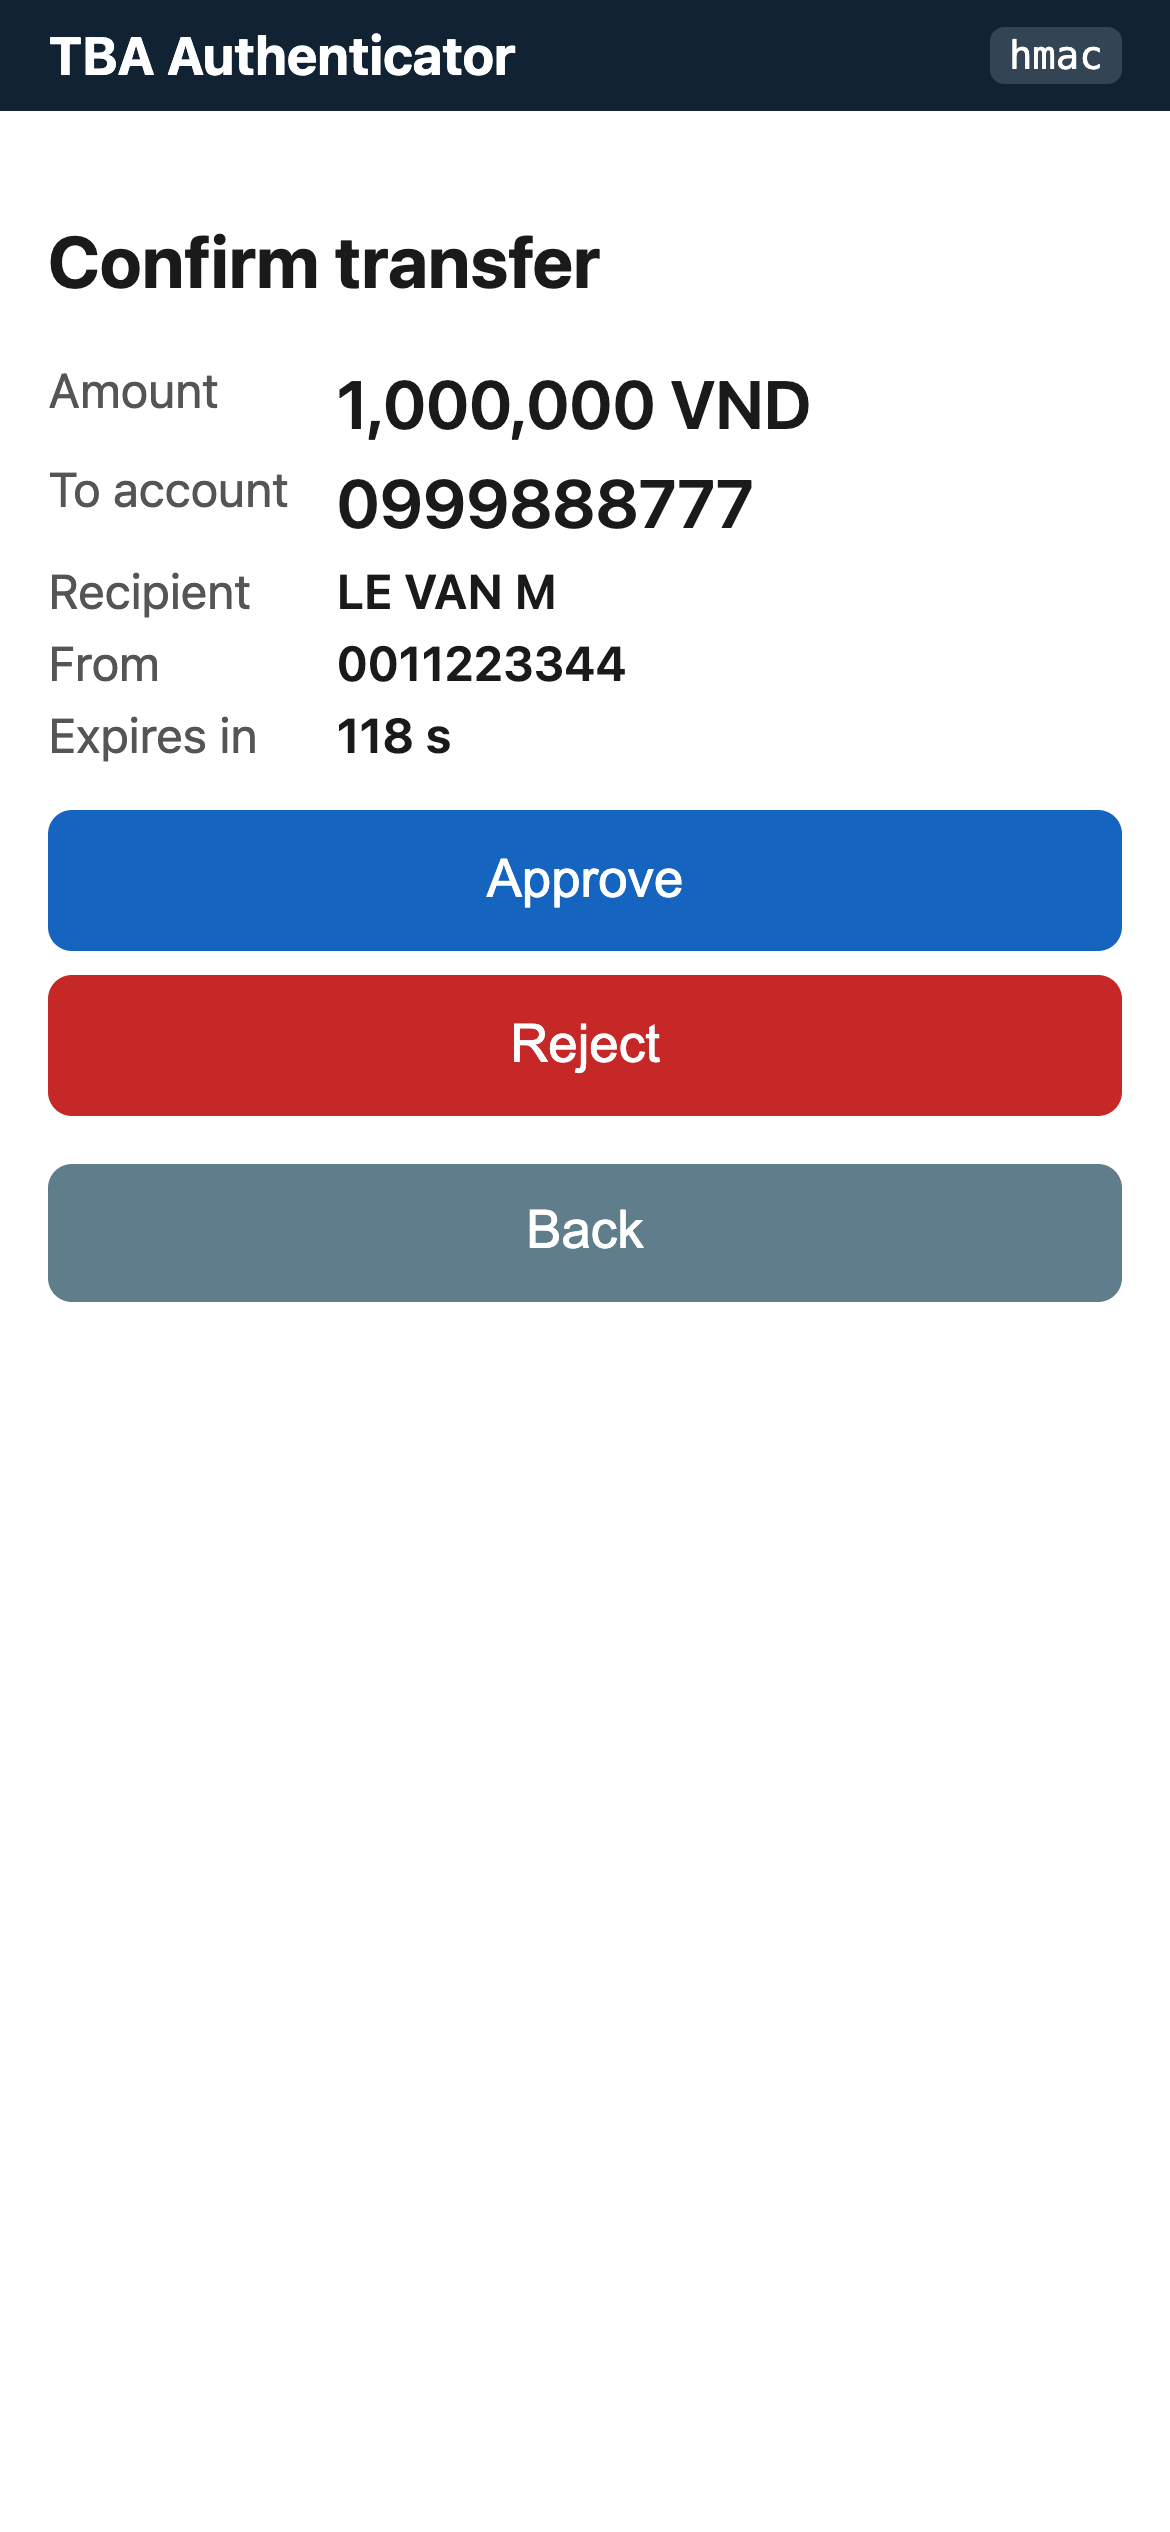
\includegraphics[height=7.5cm]{figures/hmac_phone.png}
\caption{The authenticator's confirmation screen in \texttt{hmac} mode (F7).}
\label{fig:ui}
\end{figure}
